\documentclass[book, 12pt]{article}
\usepackage[left=3cm,right=3cm,top=2cm,bottom=2cm]{geometry}
\usepackage[utf8]{inputenc}
\usepackage[russian]{babel}
\usepackage{amsmath}
\usepackage{ctex}
\usepackage{graphicx}
\usepackage{wrapfig}
\usepackage{mathtools}
\usepackage{pgfplots}
\setcounter{page}{318}
\usepackage{fancyhdr}
\pagestyle{fancy}
\fancyfoot{}
\fancyfoot[C]{\thepage}
\renewcommand{\headrulewidth}{0 mm}
\renewcommand{\footrulewidth}{0.3 mm}
\fancyhead{}

\graphicspath{ {D:\Github\Laboratory-works\LW10} }



\begin{document}
\leftskip=8cm
  Примером функции, удовлетворяющей теореме Ролля и имеющей в некоторой точке определённого знака бесконечную производную, является функция

\leftskip=10cm
\begin{equation}
	f(x) = \begin{cases}
		 \sqrt{1 - (x - 1) ^ 2},  0 <= x <= 2,\\
		-\sqrt{1 - (x - 1) ^ 2},  -2 <= x <= 0.\\
	\end{cases}
\end{equation}

\begin{wrapfigure}[1]{l}{0.3\linewidth} 
\vspace{-30ex}
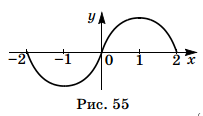
\includegraphics[width=\linewidth]{Graphic.png}
\label{fig:somelabel}
\end{wrapfigure}

\leftskip=0cm
\setlength{\parindent}{-4cm}
Эта функция непрерывна на отрезке [-2, 2], дифференцируема во всех точках
интервала (-2, 2), кроме точки x = 0, в которой f'(0) = +$\infty$ и f(-2) = f(2) (рис. 55).
В согласии с теоремой Ролля у неё имеется точка (даже две), в которой
производная равна нулю (х = $\pm$1). Графиком этой функции являются две полуокружности,
сопряжённые в точке (0; 0).

\setlength{\parindent}{1cm}
Этот пример показывает целесообразность рассмотрения в данном случае не только функций, 
имеющих конечные производные, но и функций с определённого знака бесконечными производными.

Заметим, что построением соответсвующих примеров (если, конечно, это удасться сделать) и проверяют обычно
в математике существенность тех или иных условий доказываемых теорем.

В дальнейшем мы не будем проверять необходимость условий теорем, проедоставляя это делать читателю по мере
внутренней потребности.

Из теоремы Ролля следует, что если функция непрерывна на некоторм отрезке, обращается в нуль на его концах и
дифференциируема во всех его внутренних точках, то существует его внутренняя точка, в которой производная обращается в нуль.
Короче говоря, $\textit{между двумя нулями дифференцируемой функции всегда ле-}$
$\textit{жит хотя бы один нуль её производной.}$

\setlength{\parindent}{0cm}
{\footnotesize УПРАЖНЕНИЯ. 1. Доказать, что если функция f удовлетворяет условиям теоремы Ролля на отрезке [a, b]
и не является постоянной, то на этом отрезке существуют такие точки $\xi_1$ $\xi_2$, что f'($\xi_1$) > 0 b f'($\xi_2$) < 0.\par}

{\footnotesize 2. Привести пример функции, непрерывной на отрезке [a, b] имеющей производную в каждой точке
интервала (a, b), но не имеющей производной (односторонней) в точке a.\par}

$\textbf{ТЕОРЕМА 3 (теорема Лагранжа}$\footnote[1]{Ж.-Л. Лагранж (1736-1813) - французский математик и механик.}).
$\textit{Если функция f непрерывна на отрезке}$

$\textit{$[a, b]$, и в каждой точке интервала $(a, b).$}$



\end{document}